\section{ Two body elliptical orbits:two body du grav potential  }\label{sec:q3}    
Most information for this question is found in chapter 5.10 - Relativistic effects of the reader by K. Wakker.

\bigskip

\subsection{a. The meaning of various parameters.}
The "distance-potential":
\begin{equation}
u = \frac{1}{r}
\end{equation}
Distance between both bodies:
\begin{equation}
r
\end{equation}
Angle of vector r w.r.t. reference direction
\begin{equation}
\phi
\end{equation}
Gravitational parameter \textit{(G*M)}
\begin{equation}
\mu
\end{equation}
Angular momentum:
\begin{equation}
H
\end{equation}
Speed of light in vacuum:
\begin{equation}
c
\end{equation}
Arbitrary constant to enable easy notation of first-order relativistic effects:
\begin{equation}
\alpha
\end{equation}
Relativistic effect:
\begin{equation}
3\frac{\mu}{c^2}u^2
\end{equation}
Solving the following leads to the orbital equation:
\begin{equation}
\frac{d^2u}{d\phi^2} + u = \frac{\mu}{H^2}
\end{equation}
\subsection{b. Proof of second right-hand term always being smaller than first right-hand term}
Consider the normal velocity
\begin{equation}
V_{\phi} = V \cos \Phi
\end{equation}
Consider the right-hand side of equation (1) in the question, expressed as:
\begin{equation}
\frac{\mu}{H^2} \Big[1 + 3\frac{H^2u^2}{c^2}\Big]
\end{equation}
Now for the angular momentum
\begin{equation}
H = r V_{\Phi}
\end{equation}
Rewriting (1)
\begin{equation}
\frac{d^2u}{d\Phi^2} + u = \frac{\mu}{H^2}\Big[1+3\frac{r^2V_{\Phi}^2}{c^2}\frac{1}{r^2}\Big]
\end{equation}
\begin{equation}
\frac{d^2u}{d\Phi^2} + u = \frac{\mu}{H^2}\Big[1+3\frac{V_{\Phi}^2}{c^2}\Big]
\label{proof3b}
\end{equation}
Because
\begin{equation}
V_{\Phi}^2 << c^2
\end{equation}
It is clear that
\begin{equation}
3 \frac{V_{\Phi}^2}{c^2} << 1
\end{equation}
Therefore it is stated that the second term in square brackets of eq. \ref{proof3b}, representing the term in question, is always smaller than the first term. 
\subsection{c. Finding a first-order solution for the Keplerian orbit equation}
For this, the order of successive approximation is used. 
\begin{itemize}
\item First, a zeroth-order approximation is found by neglecting the term including alpha.
\item This solution for u is substituted into the right-hand side of (1) from the question.
\item Solve the homogeneous form
\item Solve the particular form
\item Apply boundary conditions
\item Add homogeneous+particular form for the solution.
\end{itemize}
\subsection{d. Term contributions to first-order solution}
The relativistic effects are described by the second square bracket terms. 
\begin{equation}
\alpha \frac{\mu^2}{H^4}\Big[1+\frac{1}{2}e^2\Big]
\end{equation}
The above term represents a small constant term of little influence.
\begin{equation}
\alpha \frac{\mu^2}{H^4}\Big[e \Phi \sin(\Phi-\omega)\Big]
\end{equation}
The above term represents a fluctuation of which the amplitude grows larger as Phi increases.
\begin{equation}
\alpha \frac{\mu^2}{H^4}\Big[-\frac{1}{b}e^2 \cos^2(\Phi-\omega)\Big]
\end{equation}
The above term represents a pure oscillation with constant amplitude of
\begin{equation}
\frac{\alpha \mu^2 e^2}{6 H^4}
\end{equation}
Therefore, the second term which is an ever-increasing fluctuation will in the long term dominate the relativistic effect.
\subsection{e. Long-term effect approximation}
Since the first and third term in the second square brackets can be neglected, the relativistic effect is described by:
\begin{equation}
u = \frac{\mu}{H^2}\Big[1+e\cos(\Phi-\omega)\Big] + \alpha \frac{\mu^2}{H^4}e \Phi \sin(\Phi-\omega)
\end{equation}
\begin{equation}
u = \frac{\mu}{H^2}\Big[1+e\cos(\Phi-\omega)+ \alpha \frac{\mu}{H^2}e \Phi \sin(\Phi-\omega)\Big]
\end{equation}
Including the following substitution
\begin{equation}
\beta = \alpha \frac{\mu}{H^2}
\end{equation}
Leads to:
\begin{equation}
\frac{\mu}{H^2}\Big[1+e\cos(\Phi-\omega) + \beta e \Phi \sin(\Phi-\omega)\Big]
\end{equation}
Now, assuming beta is very small it is stated that
\begin{equation}
\sin \beta \Phi \approx \beta \Phi
\end{equation}
And
\begin{equation}
\cos \beta \Phi \approx 1
\end{equation}
Using both approximations it is stated that
\begin{equation}
u = \frac{\mu}{H^2}\Big[1+e\cos(\Phi-\omega)\cos(\beta \Phi) + e \sin(\Phi-\omega) \sin(\beta \Phi)\Big]
\end{equation}
The following trig-identities are used to achieve the solution:
\begin{equation}
\cos(\alpha)\cos(\beta) = \frac{1}{2}\big[\cos(\alpha-\beta)+\cos(\alpha+\beta)\big]
\end{equation}
\begin{equation}
\sin(\alpha)\sin(\beta) = \frac{1}{2}\big[\cos(\alpha-\beta)-\cos(\alpha+\beta)\big]
\end{equation}
Therefore
\begin{equation}
u = \frac{\mu}{H^2}\Big[1+e\frac{1}{2}\big[\cos(\Phi-\omega - \beta \Phi)+\cos(\Phi-\omega + \beta \Phi)\big] + e \frac{1}{2}\big[\cos(\Phi-\omega-\beta \Phi)-\cos(\Phi-\omega + \beta \Phi)\big]\Big]
\end{equation}
\begin{equation}
u = \frac{\mu}{H^2}\Big[1 + e\cos(\Phi-\omega - \beta \Phi)\Big]
\end{equation}
Q.E.D.
\subsection{f. Motion of body i}
\begin{figure}[h]
\centering
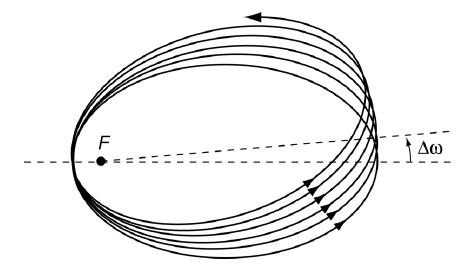
\includegraphics[scale=1]{chapters/Capture.png}
\caption{Relativistic precession of the orbit's major axis, figure 5.10 from Wakker}
\end{figure}
Given that
\begin{equation}
p = \frac{H^2}{\mu}
\end{equation}
And
\begin{equation}
u = \frac{1}{r}
\end{equation}
Using the solution from subquestion (e) the following can be stated:
\begin{equation}
r = \frac{p}{1+e\cos(\Phi - \omega - \beta \Phi)}
\end{equation}
Which can be interpreted as body i moving as a conic section around k, where the instantaneous argument of the pericenter is given by
\begin{equation}
\omega_{inst} = \omega + \beta \Phi
\end{equation}
\subsection{g. Relativistic change of the argument of pericenter}
After one full revolution of body i around body k, 
\begin{equation}
\Phi_1 = \Phi_0 + 2 \pi
\end{equation}
And therefore
\begin{equation}
\Delta \Phi = 2\pi
\label{3g1}
\end{equation}
Knowing from the answer of subquestion (f),
\begin{equation}
\omega_{inst} = \omega + \beta\Phi
\end{equation}
And therefore
\begin{equation}
\Delta \omega = \beta \Delta \Phi
\label{3g2}
\end{equation}
Substituting eq. \ref{3g1} into eq. \ref{3g2} results in
\begin{equation}
\Delta \omega = 2 \pi \beta
\end{equation}
Substituting beta in results in  
\begin{equation}
\Delta \omega = 6 \pi \frac{\mu^2}{H^2c^2}
\end{equation}
Q.E.D.









